%%%%%%%%%%%%%%%%%%%%%%%%%%%%%%%%%%%%%%%%%%%%%%%%%%%%%%%%%%%%%%%%%%%%%%%%%%%%%%%%
%% MASTER'S THESIS                                                            %%
%%                                                                            %% 
%% Title (en): Multi-Agent Systems and Organizations                          %%
%% Title (cs): Multiagentní systémy a organizace                              %%
%%                                                                            %%
%% Author: Bc. Lukáš Kúdela                                                   %%
%% Supervisor: Prof. RNDr. Petr Štěpánek, DrSc.                               %%
%%                                                                            %%
%% Academic year: 2011/2012                                                   %%
%%%%%%%%%%%%%%%%%%%%%%%%%%%%%%%%%%%%%%%%%%%%%%%%%%%%%%%%%%%%%%%%%%%%%%%%%%%%%%%%

\section{O\&P}

% O&P - authors
This section introduces the \textit{O\&P} metamodel\footnote{The metamodel was not given a name by its authors. In this thesis, we will call it \textit{O\&P}.} \cite{Odell01}, \cite{Parunak02}, \cite{Odell03b}, \cite{Odell04b} and \cite{Odell05}, put forward in 2001 by James J. Odell, H. van Dyke Parunak and their colleagues.
% Citation
The overview presented here is extracted from the most complete paper on \textit{O\&P} \cite{Odell05}.

%% O&P %%%%%%%%%%%%%%%%%%%%%%%%%%%%%%%%%%%%%%%%%%%%%%%%%%%%%%%%%%%%%%%%%%%%%%%%%

%%%%%%%%%%%%%%%%%%%%%%%%%%%%%%%%%%%%%%%%%%%%%%%%%%%%%%%%%%%%%%%%%%%%%%%%%%%%%%%%
\subsection{Integrated Metamodel}

% Integrated model - about
Figure~\ref{figure:onp-metamodel} shows the integrated metamodel proposed in \cite{Odell05}.
The following subsections will focus on parts of the integrated metamodel that can be studied in isolation.
We present the full metamodel before discussing its parts so that the reader can follow the discussion knowing how each part fits into the big picture.

% Figure: O&P metmodel
\begin{figure}[ht]
	\centering
	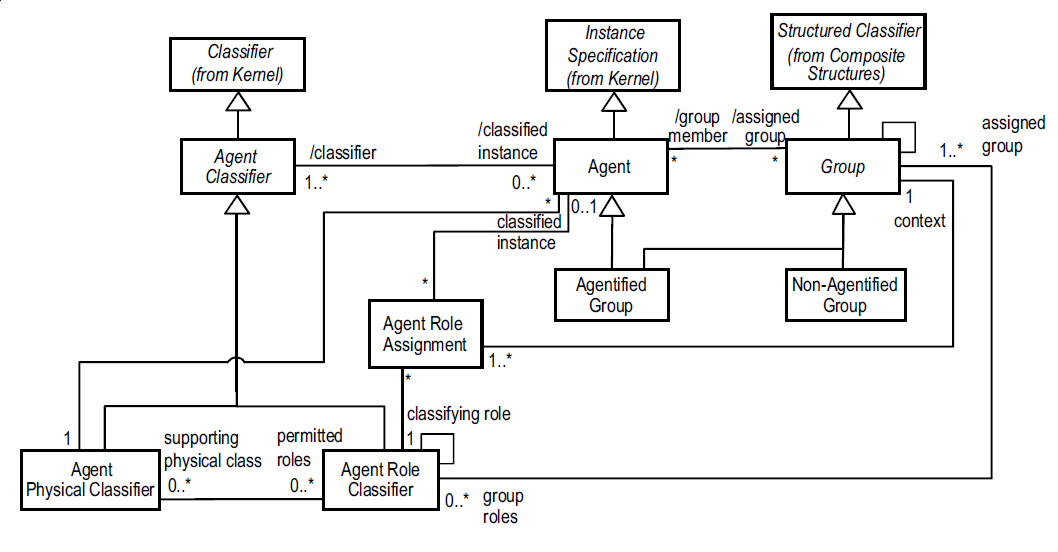
\includegraphics[width=\textwidth]{images/onp/onp-metamodel.png}
	\caption{The integrated \textit{O\&P} metamodel \cite{Odell05}}
	\label{figure:onp-metamodel}
\end{figure}

% UML Classifier vs. UML Class
To understand the integrated metamodel, it is essential to differentiate between the \textit{Classifier} and \textit{Class} UML classes.
In short, \textit{Classifier} does not have the features associated with a OOP class (e.g. the extended class, the list of implemented interfaces or attributes), while \textit{Class}, obviously, has them.
\textit{Class} is in fact a specialization of \textit{Classifier}.
It is important to make this distinction, because the agent classification is based on an extension of \textit{Classifier}, not \textit{Class}.
The reason for this is that the authors did not want to impose object-orientation upon their metamodel.
After all, it is not at all expected of an agent to exhibit behaviour intrinsic to an object, such as polymorphism.

%%%%%%%%%%%%%%%%%%%%%%%%%%%%%%%%%%%%%%%%%%%%%%%%%%%%%%%%%%%%%%%%%%%%%%%%%%%%%%%%
\subsection{Agent Classifiers and Agent Model}

\subsubsection*{Agent Classifier}

\textit{Agent Classifier} is a UML \textit{Classifier} that specifically provides a way to classify agent instances by a set of features that they have in common \cite{Odell05}.
Classification is important because it enables a common definition of a set of entities that are in some sense similar, i.e. share some features and/or capabilities.

Figure~\ref{figure:onp-agent-classifiers} shows \textit{Agent Classifier} and its two specializations: \textit{Agent Physical Classifier} and \textit{Agent Role Classifer}.

\begin{figure}[ht]
	\centering
	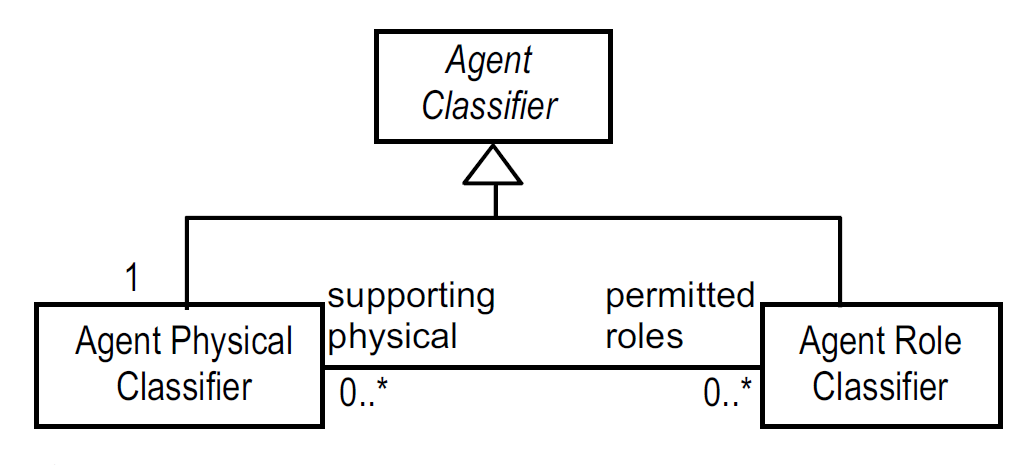
\includegraphics[width=0.6\textwidth]{images/onp/agent-classifiers.png}
	\caption{\textit{Agent Classifier} and its two specializations: \textit{Agent Physical Classifier} and \textit{Agent Role Classifier} \cite{Odell05}}
	\label{figure:onp-agent-classifiers}
\end{figure}

\subsubsection*{Agent Physical Classifier}

% Physical classifier - definition
The purpose of \textit{Agent Physical Classifier} is to define a set of features that an agent classified with it has independent of roles it plays \cite{Odell05}.
Every agent must be classified with exactly one physical classifier\footnote{Compare this with OOP, where every object must be an instance of exactly one class.} and is never reclassified during its lifetime.

% Physical classifiers vs. role classifiers
In contract to role classifiers, physical classifiers attribute primary and permanent features to agents.
Examples of physical classifiers from the real world are \textit{Human}, \textit{Male} or \textit{Female}.

Figure~\ref{figure:onp-physical-classifier-examples} shows some examples of physical classifiers forming a small class hierarchy.
Notice the \stereotype{agent physical classification} stereotype.

% Figure: Physical classifer examples
\begin{figure}[ht]
	\centering
	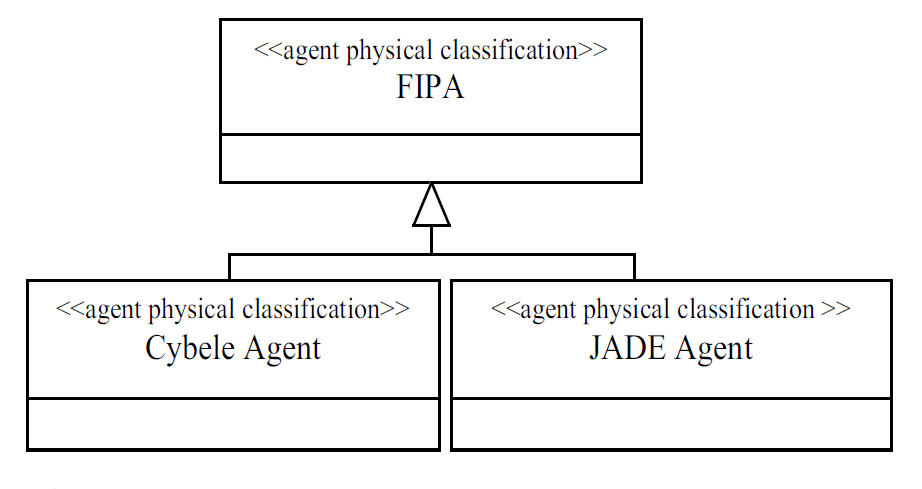
\includegraphics[width=0.5\textwidth]{images/onp/physical-classifier-examples.png}
	\caption{Examples of physical classifiers forming a class hierarchy \cite{Odell05}}
	\label{figure:onp-physical-classifier-examples}
\end{figure}

\subsubsection*{Agent Role Classifier}

% Role classifier - definition
\textit{Agent Role Classifier} is a classifier that defines a set of features that an agent classified with it acquires.
An agent can be classified with more than one role classifier at once (\textit{multiple classification}) and can be reclassified over time (\textit{dynamic classification}).

In comparison to physical classifiers, role classifiers ascribe secondary and transient features to agents.
An example of a role classifier from the real world would be \textit{Chess player}.

% Role hierarchy vs. class hierarchy
Figure~\ref{figure:onp-role-classifier-examples} depicts a small class hierarchy of role classifiers.
Notice the \stereotype{agent role} stereotype.

% Figure: Role classifer examples
\begin{figure}[ht]
	\centering
	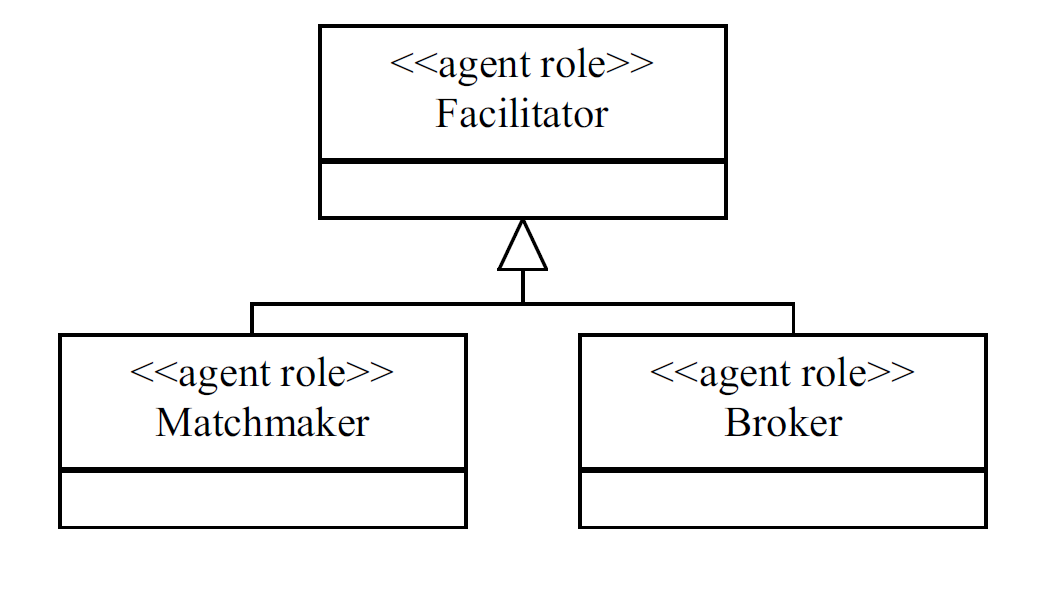
\includegraphics[width=0.5\textwidth]{images/onp/role-classifier-examples.png}
	\caption{Examples of role classifiers forming a class hierarchy \cite{Odell05}}
	\label{figure:onp-role-classifier-examples}
\end{figure}

\subsubsection*{Agent}

In \textit{O\&P}, the basic concepts are \textit{Agent Classifier} and \textit{Agent}.
These modelling constructs are considered fundamental, because they enable a MAS designer to model agents classes and agent instances respectively.
Agent classes are the design-time constructs providing the classification of the run-time constructs---agent instances.

\subsubsection*{Association between Agent Physical Classifier and Agent Role Classifier}

The association between \textit{Agent Physical Classifier} and \textit{Agent Role Classifier} specifies which role classifiers are permitted for each physical classifier, independent of the capabilities of the individual agents classified with that particular physical classifier \cite{Odell05}.

Figure~\ref{figure:onp-physical-classifier-role-classifier-association} illustrates this association.
It can be interpreted as follows. \textit{Jade} agents can play the \texttt{Broker} and \texttt{Manager} roles, and \textit{Cybele} agents can take on the role of \texttt{Broker}, \texttt{Trust Manager} and \texttt{Buyer}.

% Figure: Agent physical classifier <---> Agent role classifier association
\begin{figure}[ht]
	\centering
	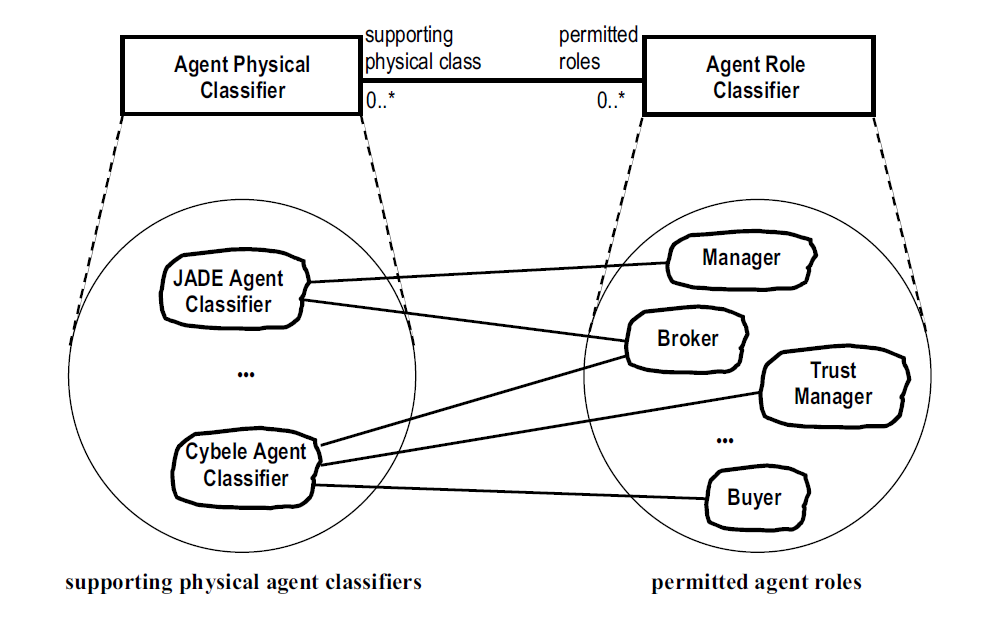
\includegraphics[width=0.8\textwidth]{images/onp/physical-classifier-role-classifier-association.png}
	\caption{The association between \textit{Agent Physical Classifier} and \textit{Agent Role Classifier} \cite{Odell05}}
	\label{figure:onp-physical-classifier-role-classifier-association}
\end{figure}

\subsubsection*{Association between Agent and Agent Classifier}

The association between \textit{Agent} and \textit{Agent Classifier} defines agents' features.
Each agent classifier classifies an agent as a member of a set of agents sharing some physical or role-related features.

% Physical vs. role classification
There are two main differences between the physical and role classification. First, the role classification is \textit{multiple} whereas the physical classification is \textit{single}.
While an agent can be classified with more than one (or even none) role classifiers at the same time, it must be classified with exactly one physical classifiers.
Second, the role classification is \textit{dynamic} in contrast to physical classification, which is \textit{static}.
Dynamic classification means that an agent can be declassified or reclassified with another role after the initial classification; static classification is invariant in time.

Figure~\ref{figure:onp-agent-agent-classifier-association} illuminates this association.
It can be read as follows. \texttt{Agent1}, a \textit{Jade} agent, is a \texttt{Manager}; \texttt{Agent2}, a \textit{Cybele} agent, is a \texttt{Manager} and \texttt{Buyer}; \texttt{Agent3}, another \textit{Cybele} agent, is a \texttt{Trust Manager}; and \texttt{Agent4}, also a \textit{Cybele} agent, is a \texttt{Broker}.

% Figure: Agent <---> Agent Classifier association
\begin{figure}[ht]
	\centering
	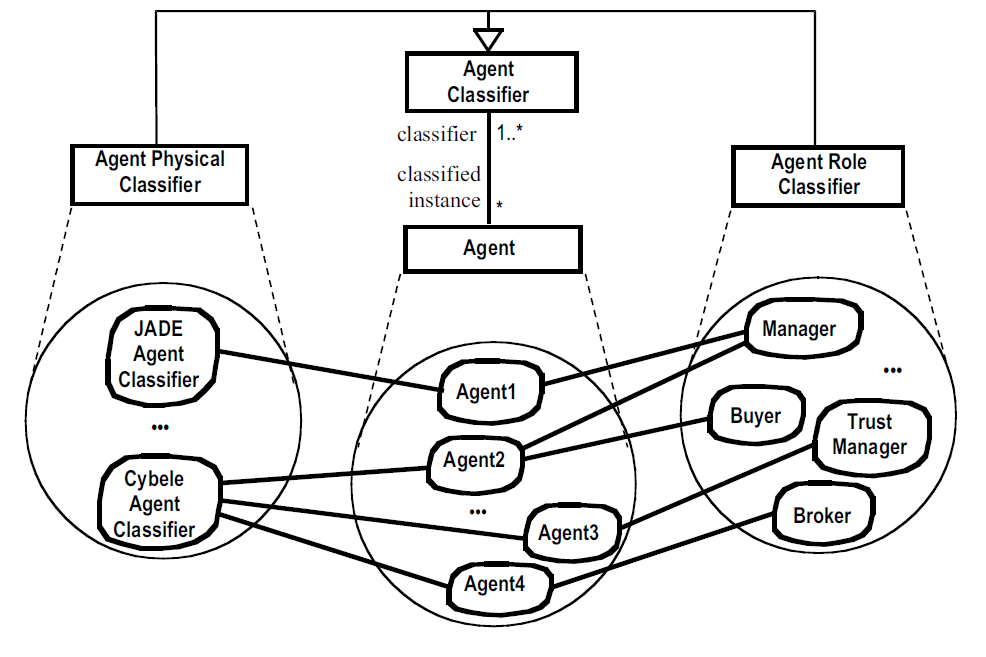
\includegraphics[width=0.8\textwidth]{images/onp/agent-agent-classifier-association.png}
	\caption{The association between \textit{Agent} and \textit{Agent Classifiers} \cite{Odell05}}
	\label{figure:onp-agent-agent-classifier-association}
\end{figure}

%%%%%%%%%%%%%%%%%%%%%%%%%%%%%%%%%%%%%%%%%%%%%%%%%%%%%%%%%%%%%%%%%%%%%%%%%%%%%%%%
\subsection{Group Model}

\subsubsection*{Group}

% Group - definition
A \textit{group} is a set of agents that are related via their roles, where these links must form
a connected graph within the group \cite{Odell05}.
This is the agent-centric way of lookig at a group.
Another way of to look at it is the role-centric way: a group is a composite structure consisting of interrelated roles, where each of the group's roles has a number of agent instances \cite{Odell05} playing that role.
A group can be formed to exploit the synergy of its members, resulting in an entity capable of performing operations that none of its constituents alone is capable of performing on its own.

Figure~\ref{figure:onp-group} shows the \textit{Group} class and its associations with \textit{Agent} and \textit{Role}.
The abstract \textit{Group} class extends the UML \textit{Structured Classifier}, which means that \textit{Group} is defined as composite structure\footnote{In UML, \textit{Structured Classifier} can be thought of as a structured set of classifiers. From this perspective, \textit{Group} is a structured set of \textit{Agent Role Classifiers}.}.

% Figure: Group
\begin{figure}[ht]
	\centering
	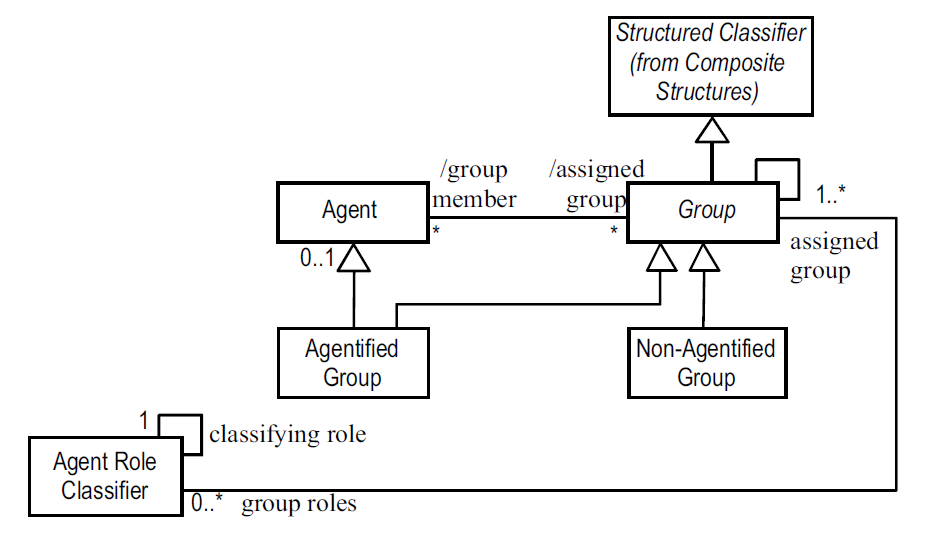
\includegraphics[width=0.8\textwidth]{images/onp/group.png}
	\caption{The \textit{Group} class and its associations \cite{Odell05}}
	\label{figure:onp-group}
\end{figure}

\subsubsection*{Association between Group and Agent}

% Association between Group and Agent
Conceptually, a group is constituted by a set of agents playing roles within that group.
The roles that the agents can play are represented by one or more agent role classifiers associated with this group.
Therefore, the set of agents forming a group can be derived from the group via the agent role classifiers \cite{Odell05}.

\subsubsection*{Association between Group and Role}

% Association between Group and Agent Role Classifier
Figure~\ref{figure:onp-group-role-association} illustrates the association between \textit{Group} and \textit{Role}.
Note that groups containing no roles are not allowed; each group must contain at least one role.
Also observe that each role has to be defined in at least one group, since roles only make sense within the context of a group.

% Figure: Group <---> Role association
\begin{figure}[ht]
	\centering
	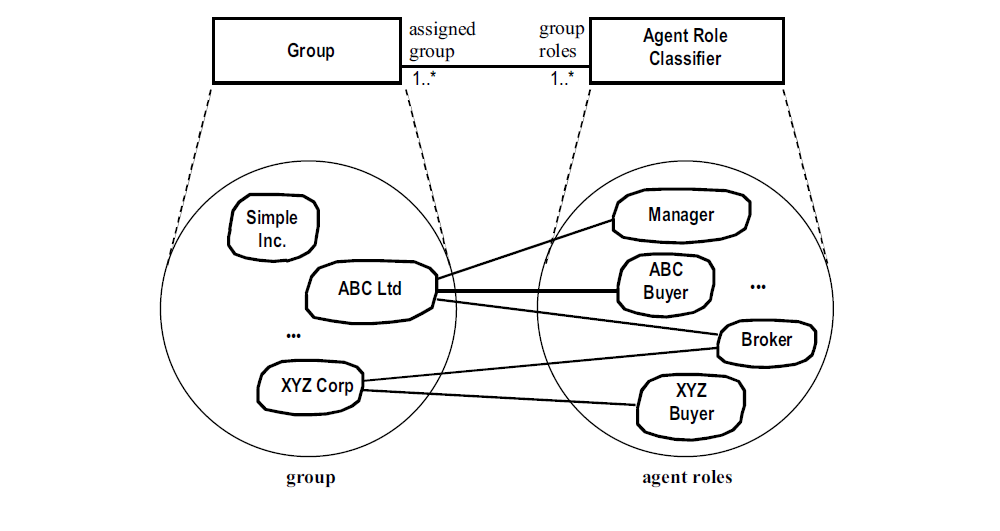
\includegraphics[width=0.8\textwidth]{images/onp/group-role-association.png}
	\caption{The association between \textit{Group} and \textit{Role} \cite{Odell05}}
	\label{figure:onp-group-role-association}
\end{figure}

\subsubsection*{Agentified and Non-Agentified Groups}

\textit{O\&P} differentiates between two types of groups: \textit{agentified}\comments{FO} and \textit{non-agentified}\comments{FO}.

% Agentified group
An \textit{agentified group} is a group that is also an agent in its own right, which means it has its own capability to interact \cite{Odell05}.
An agentified group can communicate with other agents (or agentified groups) directly, i.e. without a representative agent.
It can also be a member of other groups (agentified or not) and play roles like any other agent.
To achieve this in \textit{O\&P}, \textit{Agentified Group} is a subclass of both the \textit{Group} and \textit{Agent} classes.
Figure~\ref{figure:onp-agentified-group} shows an example of an agentified group.
Notice the \stereotype{agent} stereotype used to mark the group as agentified.

% Figure: agentified group
\begin{figure}[ht]
	\centering
	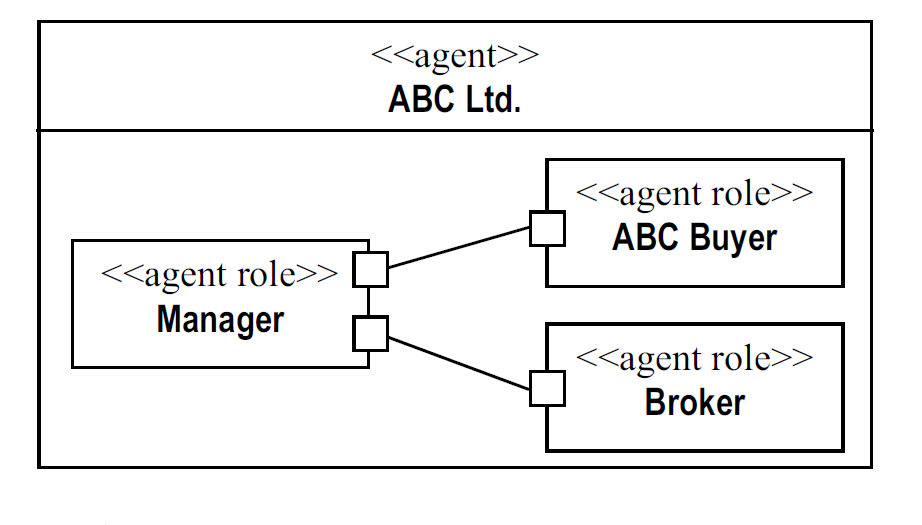
\includegraphics[width=0.5\textwidth]{images/onp/agentified-group.png}
	\caption{An example of an agentified group \cite{Odell05}}
	\label{figure:onp-agentified-group}
\end{figure}

% Non-agentified group
A \textit{non-agentified group}, while still being a first-class citizen, is not an agent in and of itself, meaning it has no capability to interact of its own.
A non-agentified group always communicates with other agents (including agentified groups) through one of its members acting as an intermediary.
This is achieved in \textit{O\&P} by \textit{Non-Agentified Group} subclassing only the \textit{Group} class and not the \textit{Agent} class.
An example of a non-agentified group is shown in figure~\ref{figure:onp-non-agentified-group}.
Notice the absence of the \stereotype{agent} stereotype.

% Figure: non-agentified group
\begin{figure}[ht]
	\centering
	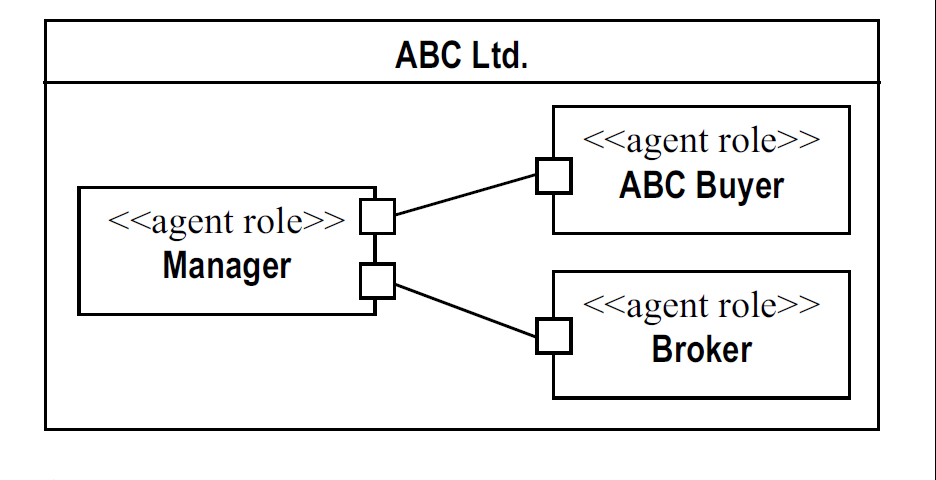
\includegraphics[width=0.5\textwidth]{images/onp/non-agentified-group.png}
	\caption{An example of a non-agentified group \cite{Odell05}}
	\label{figure:onp-non-agentified-group}
\end{figure}

%%%%%%%%%%%%%%%%%%%%%%%%%%%%%%%%%%%%%%%%%%%%%%%%%%%%%%%%%%%%%%%%%%%%%%%%%%%%%%%%
\subsection{Agent Role Assignment}

The assignment of roles to agents is dynamic, i.e. it changes in time, and is modelled by \textit{Agent Role Assignment}.
Figure~\ref{figure:onp-agent-role-assignment} shows the \textit{Agent Role Assignment} class and its associations.

% Figure: Agent Role Assignment class
\begin{figure}[ht]
	\centering
	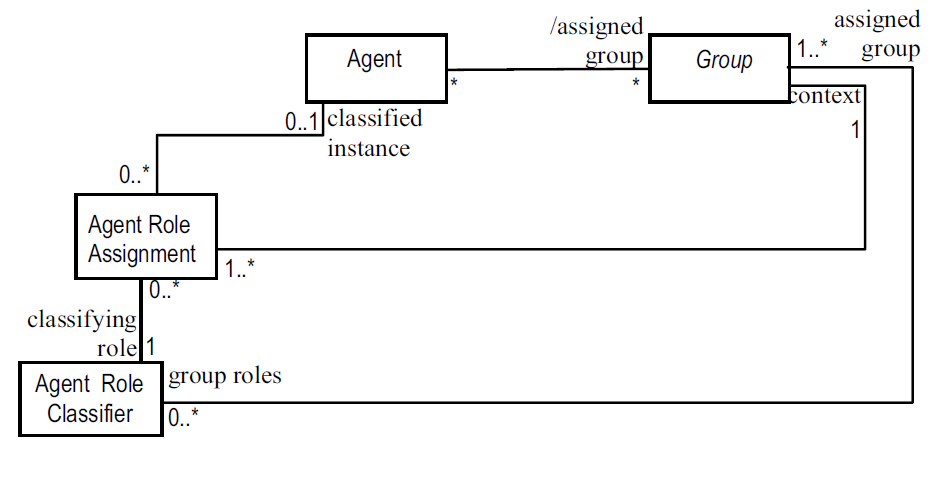
\includegraphics[width=0.8\textwidth]{images/onp/agent-role-assignment.png}
	\caption{The \textit{Agent Role Assignment} class and its associations \cite{Odell05}}
	\label{figure:onp-agent-role-assignment}
\end{figure}

\subsubsection*{Agent Role Assignment as a Ternary Association}

A model with a direct association between \textit{Agent} and \textit{Agent Role Classifier} could represent agents playing roles.
However, such model would not be able to represent a situation where an agent plays a role in one group but does not play it in another.
To model this kind of situation, it is necessary to augment the agent-to-role association with a group context.
This yields a ternary association, reified\footnote{\textit{Reification} is the process of turning an implicit abstract idea about some concept into an explicit concrete model of that concept.} in \textit{O\&P} as the \textit{Agent Role Assignment} class, whose instances link an agent to a role in a group.

\subsubsection*{Position}

It is possible to associate a group with a role leaving an agent unspecified.
Such association is called a \textit{position} and represents a situation where a concrete agent playing a role within a particular group is yet to be determined.
This turns out to be an extremely useful modelling concept, since more often than not, the organization modeller does not know (or simply does not care) which agent will actually take a particular position when the MAS is run.
Unfortunately, this association is not reified in \textit{O\&P}.
If it was reified as the \textit{Position} class, the \textit{Agent Role Assignment} class could be viewed as a reified association between the \textit{Position} and \textit{Agent} classes.